\documentclass[12pt]{article}
\usepackage[hidelinks]{hyperref}    
\usepackage[all]{hypcap}   
\usepackage{graphicx}
\graphicspath{{../images/}} % imposta path per trovare le immagini, i .. significano "la dir precedente"
\author{Andrea Malvezzi}
\title{\textbf{Architettura degli Elaboratori~-~Organizzazione Elaboratori}}  % textbf = testo bold
\date{25 Settembre, 2024}
\author{Andrea Malvezzi}
\begin{document}
\maketitle
\pagebreak
\tableofcontents
\pagebreak
\section{Il modello Von Neumann}
Tutti i PC moderni seguono un modello chiamato "Von Neumann",\\
basato sull'impiego della memoria non solo per salvare i dati ma anche per l'esecuzione di programmi.\\
Questi sono trasferiti attraverso il (sotto)bus dati e salvati in indirizzi di memoria, indicati seguentemente alla CPU dal bus indirizzi.
\subsection{I bus}
Un bus è un agglomerato di collegamenti elettrici paralleli\\
usati per trasportare informazioni da un punto A a un punto B in un sistema.
\section{La CPU}
La CPU è un componente comparabile al "cervello" di un PC, si occupa di eseguire i programmi nella memoria centrale.\\
Questa è composta da:
\begin{itemize}
    \item \textbf{CU} (control unit) , che legge e interpreta le istruzioni;
    \item \textbf{ALU} (Arithmetic Logic Unit), che esegue le operazioni (es. \textit{AND}, \textit{addizioni}, ...);
    \item i \textbf{registri}, dove vengono salvati i risultati temporanei.
\end{itemize}
\subsection{Alcuni registri importanti}
\begin{itemize}
    \item \textbf{PC} (Program Counter): indica la prossima istruzione in memoria;
    \item \textbf{IR} (Instruction Register): memorizza l'istruzione che si sta per eseguire;
    \item \textbf{MAR} (Memory Address Register): salva l'indirizzo in memoria della prossima Read/Write;
    \item \textbf{MDR} (Memory Data Register): comunica col bus dati;
    \item \textbf{PSW} (Program Status Word): "meta data" sull'ultima istruzione eseguita.
\end{itemize}
\section{Il ciclo FDE}
Il ciclo \textbf{Fetch-Decode-Execute} è diviso in tre fasi:
\begin{itemize}
    \item acquisizione dalla memoria di un'istruzione. Qui:
    \begin{itemize}
        \item il contenuto del registro PC viene scritto sul MAR e viene attivata la Read;
        \item il contenuto nell'indirizzo scritto nella MAR viene scritto\\
            sul MDR;
    \end{itemize}
    \item identificazione del tipo di operazione da eseguire. Qui:
    \begin{itemize}
        \item il contenuto di MDR viene copiato su IR;
    \end{itemize}
    \item effettuazione operazioni corrispondenti all'istruzione da eseguire. Qui:
    \begin{itemize}
        \item l'istruzione viene eseguita dall'ALU;
        \item gli eventuali operatori vengono caricati nei registri\\
            tramite MAR~/~MDR;
        \item al termine dell'esecuzione il risultato ottenuto viene spostato sul registro di destinazione.\\
            Se serve si scrive in memoria con MAR~/~MDR e linea Write.
    \end{itemize}
\end{itemize}
Al termine di questo ciclo, ricomincia da capo.
\section{La Control Unit}
Una CU si può realizzare puramente come HW con istruzioni prefissate\\
(costoso) o come HW con una parte di microprogrammazione,\\
per rendere la CPU più versatile.
\section{La Arithmetic Logic Unit}
L'ALU risiede in una parte della CPU chiamata \textbf{Data path}, assieme ai suoi componenti I/O.\\
Questo agglomerato viene utilizzato durante la fase di \textit{execute} del ciclo FDE, creando un nuovo loop detto "data path loop", governato da un \textbf{clock}.
\subsection{Il clock}
Un clock equivale ad $1/F$, con $F =:$ Frequenza di lavoro della CPU, misurata in $Hz$.\\
La frequenza equivale al numero di cicli svolti in un secondo.\\
Il ciclo di clock equivale alla durata del ciclo di data path, il quale verrà eseguito un numero di volte pari alla quantità di istruzioni da svolgere in un programma.\\
Questa nuova durata viene chiamata \textbf{"durata dell'istruzione ISA"}.
\section{Configurazioni CISC e RISC}
La microprogrammazione permise di realizzare due tipi di Computer:
\begin{itemize}
    \item \textbf{CISC}: Complex Instruction Set Computer;
    \item \textbf{RISC}: Reduced Instruction Set Computer, capace di eseguire istruzioni più semplici in meno tempo, talvolta evitando la microprogrammazione;
\end{itemize}
La prima configurazione mette enfasi sull'HW, mentre la seconda sul SW.\\
Ecco spiegato come si può realizzare una microarchitettura in entrambe le modalità.
\pagebreak
\section{Migliorare le prestazioni}
\subsection{Pipelining}
Il pipelining è una tecnica che permette di eseguire in parallelo più istruzioni (cicli FDE), usando parti diverse della CPU.
\begin{figure}[!htb]
    \centering
    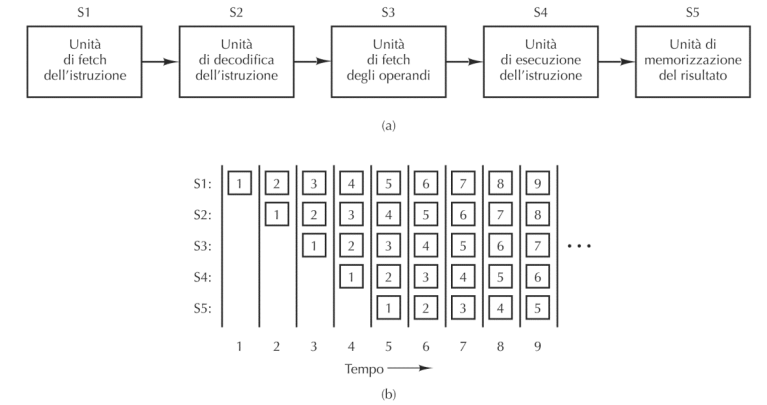
\includegraphics[width=1\textwidth, height=.7\textheight,keepaspectratio]{organizzazione_elab/pipelining.png} % essenzialmente resiza l'immagine
    \begin{center}
        \caption{\label{fig:pipelining_img}Un esempio di pipelining.} % label fuori da caption spesso non va, mettilo dentro
    \end{center}
\end{figure}
\subsection{Multicore}
In una CPU si possono simulare multiple CU e ALU per eseguire più\\
istruzioni alla volta, \textbf{in parallelo}.
\pagebreak
\subsection{Diverse forme di parallelismo}
Esistono 3 grandi tecniche per sfruttare il parallelismo, ovvero:
\subsubsection{Gli array computer}
Più processori eseguono la stessa istruzione su dati diversi.\\
Questa configurazione è detta \textbf{SIMD}: Single Instruction-stream, Multiple Data-stream.
\begin{figure}[!htb]
    \centering
    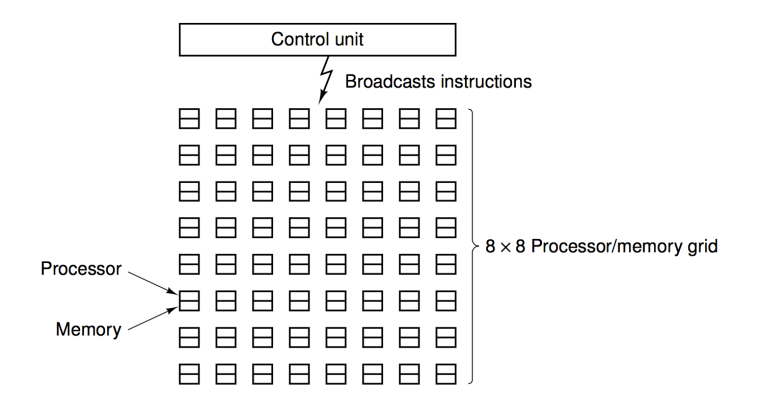
\includegraphics[width=1\textwidth, height=.7\textheight,keepaspectratio]{organizzazione_elab/array_computer.png} % essenzialmente resiza l'immagine
    \begin{center}
        \caption{\label{fig:array_computer}Negli Array Computer, ogni processore esegue la stessa istruzione, ma ha una sua memoria personale.} % label fuori da caption spesso non va, mettilo dentro
    \end{center}
\end{figure}
\pagebreak
\subsubsection{Multiprocessori}
Molti processori condividono una memoria e possono eseguire istruzioni diverse tra loro.\\
Questa configurazione è detta \textbf{MIMD}: Multiple instruction-stream, Multiple data-stream.
\begin{figure}[!htb]
    \centering
    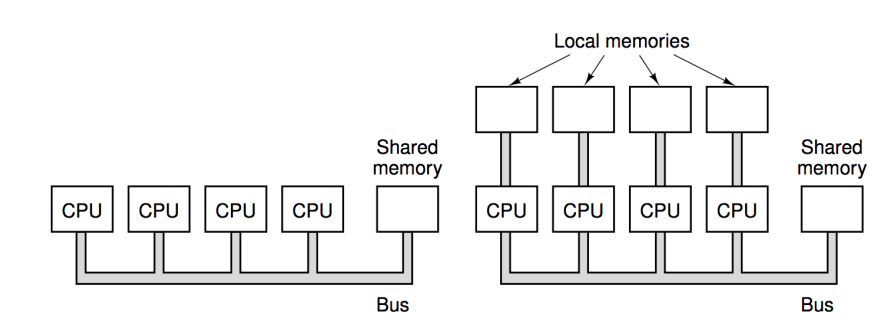
\includegraphics[width=1\textwidth, height=.7\textheight,keepaspectratio]{organizzazione_elab/multicore.png} % essenzialmente resiza l'immagine
    \begin{center}
        \caption{\label{fig:multicore}In questa configurazione i core possono avere o non avere una memoria locale, ma ne condivideranno sempre una.} % label fuori da caption spesso non va, mettilo dentro
    \end{center}
\end{figure}
\pagebreak
\subsubsection{Multicomputer}
Infine ci sono i Multicomputer, dove si hanno svariati PC che non condividono una memoria e che comunicano scambiandosi messaggi.
\begin{figure}[!htb]
    \centering
    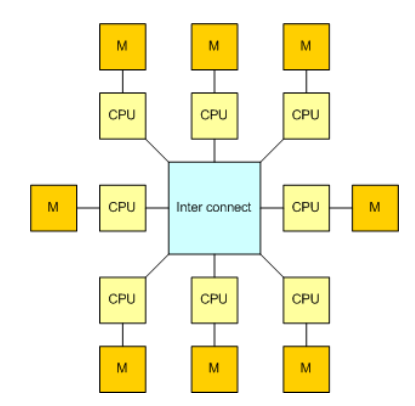
\includegraphics[width=.7\textwidth, height=.7\textheight,keepaspectratio]{organizzazione_elab/multicomputer.png} % essenzialmente resiza l'immagine
    \begin{center}
        \caption{\label{fig:multicomputer}Esempio di configurazione Multicomputer.} % label fuori da caption spesso non va, mettilo dentro
    \end{center}
\end{figure}
\pagebreak
\section{Le memorie}
Esistono tipi di memoria diversi:
\begin{itemize}
    \item volatile: il dato rimane fino allo spegnimento del dispositivo;
    \item persistente: il dato rimane anche quando si spegne il dispositivo;
    \item on-line: i dati sono sempre accessibili;
    \item off-line: la memoria deve essere montata per accedere ai dati al suo interno;
\end{itemize}
\begin{figure}[!htb]
    \centering
    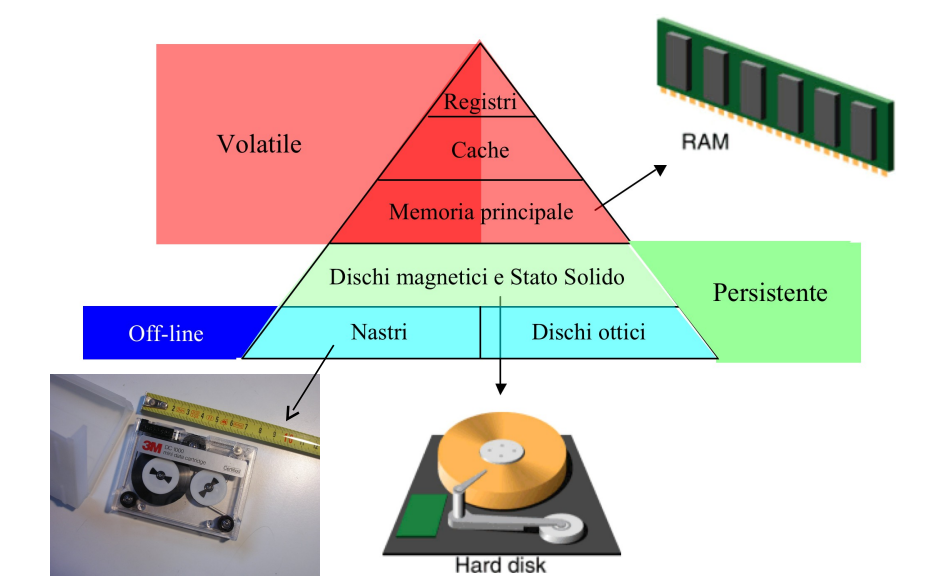
\includegraphics[width=.9\textwidth, height=.7\textheight,keepaspectratio]{organizzazione_elab/memorie.png} % essenzialmente resiza l'immagine
    \begin{center}
        \caption{\label{fig:tipi_memoria}Salendo aumenta il costo per byte.} % label fuori da caption spesso non va, mettilo dentro
    \end{center}
\end{figure}
\pagebreak
\subsection{Salvare in memoria}
La memoria è divisa in banchi da 8 byte ma ovviamente i computer \\
lavorano con dati molto più grandi di così.
Per salvare questi dati in memoria, li si "frammenta" nei loro byte e questi si salvano seguendo due filosofie:
\begin{itemize}
    \item big endian: assegnando indirizzi da sx a dx (dal byte con valore inferiore a quello di valore maggiore);
    \item little endian: assegnando indirizzi da dx a sx (dal byte con valore maggiore a quello di valore inferiore);
\end{itemize}
\subsection{La memoria cache}
La cache è una memoria poco capiente ma veloce, che si usa per salvare dati a cui si accede di frequente.\\
Quando la CPU necessita di un dato, lo cerca nella cache e se non lo trova riprova nella memoria, per poi caricarlo se l'operazione termina con esito positivo.
\subsubsection{Il principio di località}
Quando si accede alla memoria più volte in uno span di tempo corto, è probabile che si stia accedendo a blocchi di memoria contigui.\\
Per questo motivo si caricano spesso zone di memoria contigue all'interno della cache: così facendo aumenta la probabilità di risparmiare tempo con gli accessi successivi.
\pagebreak
\subsection{Gli Hard Disk (HD)}
Un HD è un dispositivo elettro-magnetico per salvare dati.\\
Possiede diverse parti:
\begin{itemize}
    \item testina: componente montato su un braccio detto "di accesso", usato per scrivere sui piatti del disco;
    \item traccia: sequenza circolare di bit sui piatti;
    \item settore: porzione di traccia contenente \textit{n} bit.
\end{itemize}
\begin{figure}[!htb]
    \centering
    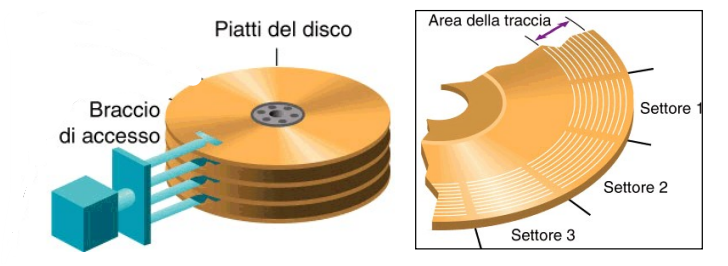
\includegraphics[width=.9\textwidth, height=.7\textheight,keepaspectratio]{organizzazione_elab/hd.png} % essenzialmente resiza l'immagine
    \begin{center}
        \caption{\label{fig:hd_struttura}Composizione di un HD.} % label fuori da caption spesso non va, mettilo dentro
    \end{center}
\end{figure}
\subsection{Memorie allo stato solido}
Sono dispositivi completamente elettronici, quindi anche più resistenti (si ha un'assenza di componenti meccaniche) e veloci, ma meno capienti.
\pagebreak
\subsection{Memoria RAID}
Per ridurre il gap di velocità tra CPU e memoria, si è pensato di utilizzare più dischi in parallelo.\\
Tale configurazione è detta RAID, e si suddivide in 5 livelli:
\begin{itemize}
    \item livello 0: Non-reduntant data striping. Si hanno più dischi che salvano blocchi di dati (stripes) diversi, senza backup;
    \item livello 1: Redundant data striping. Come il livello 0, ma con backup;
    \item livello 2: Data striping at bit level. Spezza i dati in bytes piuttosto che in blocchi;
    \item livello 3: Bit-interleaved parity. Come il precedente, ma con un bit di parità per il controllo dell'errore;
    \item livello 4: Block-interleaved parity. Come il livello 0, ma con bit di parità;
    \item livello 5: Block-interleaved distributed parity. Come il precedente, ma i bit di parità sono disposti su più dischi per evitare errori.
\end{itemize}
\subsection{CD}
I CD sfruttano un principio ottico: sono composti da zone piane (land) e forate (pit) e in base alla sequenza con cui vengono lette dal PC, queste rappresentano 0 oppure 1.
\section{Le schede grafiche}
Le GPU possono essere programmate in appositi linguaggi (come CUDA-C) per diventare in grado di eseguire programmi non grafici (vedi \textit{miners di Bitcoin}).
\section{Conclusioni}
Come dimostrato, i PC sono composti da più componenti, ognuno dei quali svolge un compito unico e comunica con gli altri mediante BUS, ai quali si collegano grazie ad un \textbf{controller} e ad un \textbf{arbitro} (per evitare di utilizzarne uno al contempo stesso).
\end{document}